% Geometric Fields Mechanics: Sigma Construction
% Author: Antonio miti

\documentclass[border=10pt]{standalone}
\usepackage{tikz}


\usetikzlibrary{arrows,positioning}
\tikzset{%
  % Specifications for style of arrows:
   projection/.style={
           ->,
           shorten <=1pt,
           shorten >=1pt,},
   lagmap/.style={
           projection,
           red},
   hammap/.style={
           projection,
           blue},
   inclusion/.style={
   		   left hook->,
           shorten <=1pt,
           shorten >=1pt,},                            
  % Specifications for style of nodes:
   base/.style = {rectangle, rounded corners, draw=black,
                  minimum width=2cm, minimum height=1cm,
                  text centered, font=\sffamily},
   tangent/.style = {circle, rounded corners, draw=black,
                  minimum width=3cm, minimum height=1cm,
                  text centered, font=\sffamily},
      tangent/.style = {circle, rounded corners, draw=black,
                  minimum width=2cm, minimum height=1cm,
                  text centered, font=\sffamily},               
   verticalsmall/.style = {rectangle, rounded corners, draw=black,
                  minimum width=2cm, minimum height=1cm,
                  text centered, font=\sffamily},
   verticalbig/.style = {rectangle, rounded corners, draw=black,
                  minimum width=1cm, minimum height=1cm,
                  text centered, font=\sffamily},                              
   hamiltonian/.style = {base, fill=blue!20},
   lagrangian/.style = {base, fill=red!20},
   process/.style = {base, minimum width=1cm,
                     font=\ttfamily},
}

\begin{document}    

% Drawing part, node distance is 1.5 cm and every node
% is prefilled with white background

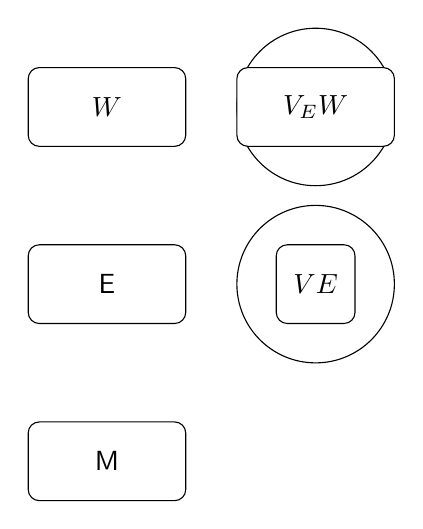
\begin{tikzpicture}[node distance=2.25cm,
    every node/.style={fill=white, font=\sffamily}, align=center]

  % Specification of nodes (position, etc.)
  \node (M_block)	[base]	{M};
  \node (E_block)	[base, above of= M_block]	{E};
  \node (W_block)	[base, above of= E_block]	{$W$};
  \node (TE_block)	[tangent, right of= E_block, , xshift=0.4cm]	{$TE$};
  \node (VE_block)	[process, right of= E_block, , xshift=0.4cm]	{$VE$};

  \node (TW_block)	[tangent, right of= W_block, , xshift=0.4cm]	{$TW$};
  \node (VmW_block)	[verticalbig, right of= W_block, , xshift=0.4cm]	{$V_MW$};
  \node (VeW_block)	[verticalsmall, right of= W_block, , xshift=0.4cm]	{$V_EW$};

  \end{tikzpicture}
  
  
  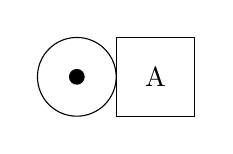
\begin{tikzpicture}
    \node[matrix] (A) {
        \draw (0,0) rectangle (1,1); 
        \node at (0.5,0.5) {A}; \\
    };
    \node[matrix,left of=A] (B) 
    {
        \draw (0.5,0.5) circle (0.5);
        \fill (0.5,0.5) circle (0.1); \\
    };
\end{tikzpicture}
\end{document}